\documentclass[11pt, a4paper,english,spanish]{article}
\usepackage[spanish]{babel}
\usepackage[utf8]{inputenc}
\parskip = 11 pt
\usepackage[width=18cm, left=1.5cm, top=2.25cm, height= 25cm]{geometry}

\usepackage{amsmath}
\usepackage{algorithm}
\usepackage[noend]{algpseudocode}
\usepackage{amsfonts}
\usepackage{amssymb}
\usepackage{fancyhdr}
\usepackage{lastpage}
\usepackage{caratula}
\usepackage{url}
\usepackage{flafter}
\usepackage{afterpage}
\usepackage{float}
\usepackage{listings}
\usepackage{color}
\usepackage{verbatim}
\usepackage{placeins}
\usepackage{graphicx}
\usepackage{caption}
\usepackage{subcaption}
\definecolor{gray97}{gray}{.97}
\definecolor{gray75}{gray}{.75}
\definecolor{gray45}{gray}{.45}

\algdef{SE}[DOWHILE]{Do}{doWhile}{\algorithmicdo}[1]{\algorithmicwhile\ #1}%
 
\usepackage{listings}
\lstset{ frame=Ltb,
     framerule=0pt,
     aboveskip=0.5cm,
     framextopmargin=3pt,
     framexbottommargin=3pt,
     framexleftmargin=0.4cm,
     framesep=0pt,
     rulesep=.4pt,
     backgroundcolor=\color{gray97},
     rulesepcolor=\color{black},
     %
     stringstyle=\ttfamily,
     showstringspaces = false,
     basicstyle=\small\ttfamily,
     commentstyle=\color{gray45},
     keywordstyle=\bfseries,
     %
     numbers=left,
     numbersep=15pt,
     numberstyle=\tiny,
     numberfirstline = false,
     breaklines=true,
   }


% minimizar fragmentado de listados
\lstnewenvironment{listing}[1][]
   {\lstset{#1}\pagebreak[0]}{\pagebreak[0]}
 
\lstdefinestyle{consola}
   {basicstyle=\scriptsize\bf\ttfamily,
    backgroundcolor=\color{gray75},
   }
 
\lstdefinestyle{C++}
   {language=C++,
   }
 
\newcommand{\real}{\ensuremath{\mathbb{R}}}
\newcommand{\grad}{\hspace{-2mm}$\phantom{a}^{\circ}$}

\pagestyle{fancy}

\title{MotionCapture}

%Estilo para el encabezado
\fancyhead[LO, LE]{Métodos Numéricos}
\fancyhead[RO, RE]{2$^{do.}$ cuatrimestre de 2014}
\fancyhead[CO, CE]{}

\fancyfoot[CO, CE]{P\'agina \thepage\ de \pageref{LastPage}}

\begin{document}
%Estos son los parametros para la caratula
\materia{Métodos Numéricos}
\submateria{Trabajo Pr\'actico Nro. 2}
\titulo{Ranking web}
\fecha{\today}
\integrante{Martin Carreiro}{45/10}{martin301290@gmail.com}
\integrante{Kevin Kujawski}{459/10}{kevinkuja@gmail.com}
\integrante{Juan Manuel Ort\'iz de Z\'arate}{403/10}{jmanuoz@gmail.com}
\maketitle
\newpage

%Pagina de titulo e indice
\thispagestyle{empty}

\tableofcontents

%\newpage

\normalsize
\section{Resumen}

Los sitios web a medida que fueron creciendo en cantidad en la época de los 90's, se complicó el acceso a ellos y ,a menos que alguien te comentara o a través de publicidades, era muy dificil acceder a la información deseada. Es por eso que se produjo el auge de los buscadores, que a partir de palabras claves, podrían devolverte sitios que  puedan llegar a responder tu pregunta o decirte algo al respecto. 
Un primer problema de entrada, es que, como todo en la vida, la calidad de dicho contenido puede no ser el deseado y existan mejores. Durante este trabajo repasaremos 3 algoritmos conocidos de ranqueo de páginas web, veremos los resultados y los compararemos. \\
Una vez que sepamos cómo funcionan y cómo ordenan y ubican los resultados, intentaremos responder a la pregunta: cuáles son los pasos a seguir para poder mejorar tu sitio y que salga con mejor puntaje que la competencia.\\
Durante el desarrollo del trabajo práctico comprobaremos que la forma de posicionarse en las búsquedas depende, en todos los algoritmos, de los links que otras páginas tengan a tu sitio (y viceversa), por lo tanto lo que concluiremos es que si el cliente quiere posicionarse bien, en el menor tiempo posible, habrá que recomendarle que negocie con otras páginas web para ser apuntadas por estas. La diferencia es que no necesariamente serán las mismas, esto dependerá de que método de búsqueda se esté utilizando.

\newpage
\section{Introducci\'on te\'orica}

\subsection{Algoritmos de búsqueda}

Los buscadores web son aquellos sitios que dada una palabra o frase encuentran las páginas que tienen lo que el usuario estaba buscando en una gran cantidad de casos. El secreto del éxito de estos buscadores no es sólo que encuentran el sitio con la palabra o frase deseada sino que encuentran el mejor resultado para esta. \\
Esto lo hace mediante métodos de rankeo que no son nada sencillos y es por eso que estaremos analizando 3 algoritmos distintos para hacerlo: PageRank, HITS e Indeg. Describiremos la idea teórica de cada uno, sus implementaciones y analizaremos cualitativa y temporalmente sus resultados. Es decir cuanto tardan en ejecutarse y que tan buenos son los resultados devueltos para distintas búsquedas. Procedamos entonces a explicar la idea de cada uno.

\subsubsection{PageRank}

El algoritmo de búsqueda llamado \textbf{PageRank} lo desarrollaron los fundadores de Google, Page y Brin, y fue tan revolucionario que cambió la forma en que se empezó a buscar en la web. \\
El primer punto de este algoritmo es mirar a la web como un grafo dirigido, donde cada nodo representa un sitio y los vertices van de un nodo a otro si un sitio contiene un link direccionando a este otro.
A partir de esto se define una \emph{matriz de vínculos} $M$, y como su nombre lo indica, esta representará las conectividades de los sitios pero con la particularidad de que tendrá información acerca de cuanto puntaje le asigna un sitio a otro, es decir, $m_{ij}$ será 1/$G_j$  (siendo $G_j$ el grado de salida del sitio $j$) si $j$ tiene un link a $i$ y 0 en otro caso.
De esta forma, la importancia de cada sitio esta medida por la calidad de sitios que linkean a cada uno, y a su vez la calidad esta conformada por la cantidad de sitios a los que redirijo, ya que si un sitio redirige a pocos sitios a cada uno estara otorgandole un puntaje cercano al 1, y en caso contrario el puntaje que otorgará sera cercano al 0 y no tendrá mucho peso a la hora de que los sitios de destino obtengan mayor importancia gracias a este.\\
Facilmente se puede deducir que todas las columnas de la matriz resultante van a sumar 1, por lo que será una matriz \textit{``estocastica por columnas"}. Luego el problema de encontrar el ranking de cada cada sitio es equivalente a encontrar un $x\in \mathbb{R}^n$ tal que $Px = x$, es decir, encontrar (suponiendo que existe) un autovector asociado al autovalor 1 de una matriz cuadrada, tal que $x_i \ge
0$ y $\sum_{i = 1}^n x_i = 1$. 
\\
\\
Un detalle importante que se debe considerar es que para que el PageRank funcione no puede haber nodos desconectados, ya que de ser así la matriz de vínculos no sería estocastica por columnas debido a que la columna de la matriz que representa a los sitios que linkea estarían todos en 0. Por esta razón es que Bryan y Leise \cite{Bryan2006} muestran una forma 

\subsubsection{HITS}

Este algoritmo fué pensado por Kleinberg $[2]$ y su esenscia está en la separación conceptual que hace entre un nodo \textit{autoridad} y uno \textit{Hub}. Vale aclarar que en este caso también entenderemos a un nodo como parte del grafo que modela a la internet y que representa a un sitio web en particular. \\
Autoridad serían aquellos sitios que tienen mayor importancia dentro de un tema específico y Hubs los que apuntan a estos sitios. En palabras mas terrenales las autoridades serían los que tienen las mejores respuestas y los hubs los que conocen a las mejores autoridades.
En la práctica se entiende por autoridades a aquellos nodos que son apuntados por una gran cantidad de sitios y por Hubs a los nodos a apuntan a muchos otros. Una web es mejor Autoridad si es apuntada por buenos Hubs y viceversa, un Hub es mejor si apunta a las mejores autoridades.\\
Para modelarlo computacionalmente pensamos a la red como una matriz $A \in \{0,1\}^{n \times n}$ donde cada fila y columna representan a un nodo y tienen un 1 si el nodo fila apunta al nodo columna o un 0 en caso contrario. Luego Kleinberg nos señala que debemos crear un vector \textit{x} e \textit{y} para agrupar las autoridades y hubs respectivamente. Estos vectores nos dice que los obtengamos tomando un x0 e y0 inciales con todos sus valores 1 y realizando este cálculo:

\begin{eqnarray}
x & = & A^ty \label{eq:auth-update-math} \\
y & = & Ax, \label{eq:hub-update-math} 
\end{eqnarray}

n veces (para un n definido) o hasta obtener un error menor a la tolerencia deseada. El error lo obtenemos calculando la norma manhattan entre el vector obtenido en el paso actual y el previo a este (mas adelante explicaremos como es la norma esta).\\
Luego de esto nos quedan en cada vector ordenados en el vector $x$ las mejores autoridades y en el $y$ los mejores hubs.

Dicho procedimiento debe aplicarse sobre una subred (denominada root-set) que debe calcularse previamente. Para esto mediante algún buscador simple, basado en texto por ejemplo, se acota la red a una determinada cantidad de nodos. Luego se le agregan aquellos que apuntan a algún nodo de dicha sub-red y los apuntados por esta, para finalmente sí, a este root-set aplicarle HITS. En este trabajo supondremos que este acotamiento previo ya fué efectuado.


\subsubsection{Indeg}
A modo de comparación para los experimentos, agregamos este algoritmo que resulta un poco inocente. Supongamos que tenemos una red de páginas, el peso, o importancia, de cada una será el promedio de la cantidad de links existentes en otras páginas del mismo conjunto hacia esta sobre la cantidad de links en total. El cálculo del mismo es lineal en la cantidad de referencias y su complejidad espacial es un vector de tamaño igual que el conjunto inicial de páginas. Este vector final es el resultado.

\begin{center}
$[k_1/n, k_2/n, ..., k_n/n]\quad 0 \leq k_i \leq n \quad n = cantTotalLinks$
\end{center}

\subsection{Norma Manhattan}

A lo largo de esta presentación, utilizaremos la distancia L1 entre dos vectores, también llamada Norma Manhattan.
La norma Manhattan es la suma de la diferencia coordenada a coordenada en modulo:

\begin{center}
$\left \| v - w \right \|_{1} = \sum_{i=1}^{n} \left | v_{i} - w_{i} \right |$
\end{center}

El uso del mismo estará detallado en el desarrollo de cada algoritmo presentado.


\subsection{Matriz Dispersa}
   Se define como matriz dispersa a aquella a la que la mayoría de sus elementos son cero.
   Ejemplo:

   $$ 
\begin{bmatrix}
       0    &      0    &   0       &   0           &   a_{04}    \\
       0    &   a_{11}  &   a_{12}  &   0           &   0    \\
       0    &      0    &   0       &   a_{23}      &   0    \\
       0    &      0    &   0       &   a_{33}      &   0    \\
  a_{40}    &      0    &   0       &   0           &   0    \\
\end{bmatrix} 
$$


\subsection{DOK vs CRS vs CSC}
    La matriz dispersa al tener la propiedad de tener muy pocos valores no$-$cero es conveniente solo guardar estos y asumir el resto como cero. Existen varias estructuras como Dictionary of Keys (dok), Compressed Sparse Row (CSR) o Compressed Sparse Column (CSC) pensadas para optimizar el espacio y las operaciones con estas estructuras de datos. En el desarrollo de este TP, utilizamos DOK por facilidad en el uso del mismo. Tanto CSR o CSC se basan en la estructura Yale y se diferencian en como guardan los mismos valores, uno priorizando las filas y otro las columnas respectivamente.\\
    La estructura Yale consiste en a partir de la matriz original obtener tres vectores que contengan 
    \begin{itemize}
        \item A = los elementos no$-$cero de arriba-abajo,izquierda-derecha
        \item IA = los indices para cada fila i del primer elemento no-cero de dicha fila
        \item JA = los indices de columna para cada valor de A
    \end{itemize}
    Si bien el caso de que haya una fila con muchos números no-ceros es más beneficiosa la utilización de esta estructura, la facilidad con DOK permite hacer pruebas más rápido.Y nos pareció poco práctico ponernos a implementar todas las lógicas requeridas para la eliminación o agregación de nuevos datos en estas estructuras ya que no hacían a la escencia del TP y complejizaban el código y el debagueo durante las pruebas y el desarrollo. Consideramos que la optimización otorgada por DOK es suficiente para el tipo de análisis que deseamos hacer sobre los algoritmos de rankeo solicitados



\newpage
\section{Desarrollo}

A continuación detallamos cómo fue el desarrollo de los algoritmos presentados previamente

\subsection{Page Rank}
El algoritmo de PageRank lo dividimos en dos etapas, primero la inicializaci\'on en donde se crea la matriz estoc\'astica y luego la corrida en donde se itera y calcula el pagerank hasta que la diferencia de norma entre los vectores sea menor que la tolerancia establecida.

Inicializaci\'on:


\begin{algorithm}
\caption{initialize(c, dim, links)}\label{euclid}
\begin{algorithmic}[1]
\State $\textit{vectorInicial = vector(dim, 0);}$ \Comment{creo un vector de dim elementos y lo inicializo en 0}
\State $\textit{vectorInicial[0] = 1;}$ \Comment{pongo el primer elemento en 1}
\State $\textit{matriz = DOK(dim);}$ \Comment{la matriz representará al $M_f$}
\For{$cada\ link\ en\ links$}
\If{$link\ tiene\ salidas$}
\For{$cada\ salida\ del\ nodo$}
\State $\textit{;}$ \Comment{}
\EndFor
\Else
\State $\textit{desconectados.agregar(link);}$ \Comment{}
\EndIf
\EndFor


\end{algorithmic}
\end{algorithm}

Calculo del PageRank:
\begin{lstlisting}[frame=single] 
Hasta que converja:
	Multiplico la matriz por el vector actual.
	Aplico el algoritmo para tener en cuentas los nodos desconectados.
	Aplico el algoritmo para tener en cuenta el navegante aleatorio.
	Guardo el vector actual.
	
\end{lstlisting}


\subsection{HITS}
Este también lo dividimos en la etapa en la etapa de inicialización y de cálculo de sus vectores. En la primera creamos la matriz estocástica e inicializamos los vectores y en la segunda calculamos los mismos hasta que iteremos k veces o la diferencia obtenida sea menor que la tolerancia.

%Inicializaci\'on:
%\begin{lstlisting}[frame=single]  
%Creo el Dok vacio
%Para cada arista:
%	defino en el dok el nodo desde y hasta
%	
%Inicio los vectores de hubs y autoridades con todos sus valores en 1 y normalizados
	
%\end{lstlisting}

%Cálculo de vectores Hubs y Autoridades
%\begin{lstlisting}[frame=single] 
%Itero de 1 a K
%	Para el vector de hubs multiplico el dok transpuesto por el vector de autoridades y normalizo
%	Para el vector de autoridades multiplicoel dok transpuesto por el vector de hubs y normalizo
%	Si la diferencia entre el nuevo vector de hubs o autoridades con su valor previo es menor a la tolerancia termino la iteracion
%\end{lstlisting}
\subsection{Indeg}

La implementación de este algoritmo es bastante simple. Tomamos un vector inicial con ceros del tamaño de las páginas y recorremos todas las referencias de cada página hacia al resto, y por cada una de los sitios a los que visita, le sumamos en 1/cantidadLinksTotal su puntaje en el vector inicial.

\begin{lstlisting}[frame=single] 
Inicializo el vector de resultados con ceros.
Para cada conjunto de referencias de una pagina:
	Para cada referencia:
		Al vector resultados le sumo 1 / cantidad total de los links
	
\end{lstlisting}

\newpage
\section{Experimentación Y Resultados}

\subsection{Casos de prueba}
   A continuación se listarán los casos utilizados y después se compararán los resultados.

	\begin{itemize}
		\item MOVIES: Este caso incluye 5797 páginas
		\item ABORTION: Este caso incluye 2293 páginas
		\item GENETIC: Este caso incluye 3468 páginas
		\item STANFORD: Este caso incluye 281903 páginas
		\item GOOGLE: Este caso incluye 916428 páginas
	\end{itemize}   

\subsection{Comparación de Normas}

En esta sección vamos a mostrar como evoluciona la norma Manhattan (también conocida como distancia L1) entre dos vectores a medida que se suceden las iteraciones.
La norma Manhattan es la distancia entre dos vectores, o en otras palabras, la suma de la diferencia coordenada a coordenada en modulo:

\begin{figure}[h!]
   \centering
    
\includegraphics[width=0.5\textwidth]{imagenes/norma_manhattan.png}
\end{figure}


\subsubsection {PageRank}

Para evaluar el comportamiento de la norma manhattan variando la probabilidad del navegante aleatorio, el cual de ahora en más lo denotaremos como el parámetro \textbf{c}

Los casos de prueba se corrieron sin un limite entre normas pero si con un limite de 1000 iteraciones, ya que, según lo que investigamos, con un c 	$\approx$ 0.15 la matriz suele converger en un máximo de 50 iteraciones, que por lo que se puede observar suele ser proporcional esta relación a medida que aumenta el c.

A continuación se muestran los resultados para cuatro tests de como evoluciona la norma a lo largo de las iteraciones y como varía la misma con distintos c, y que luego discutiremos más adelante.
Cabe aclarar que expresamos los valores de la norma en escala logarítmica para una mejor visualización y para que se obtenga un mejor entendimiento de como disminuye de a varias magnitudes en cada iteración.


\begin{figure}
\begin{center}
       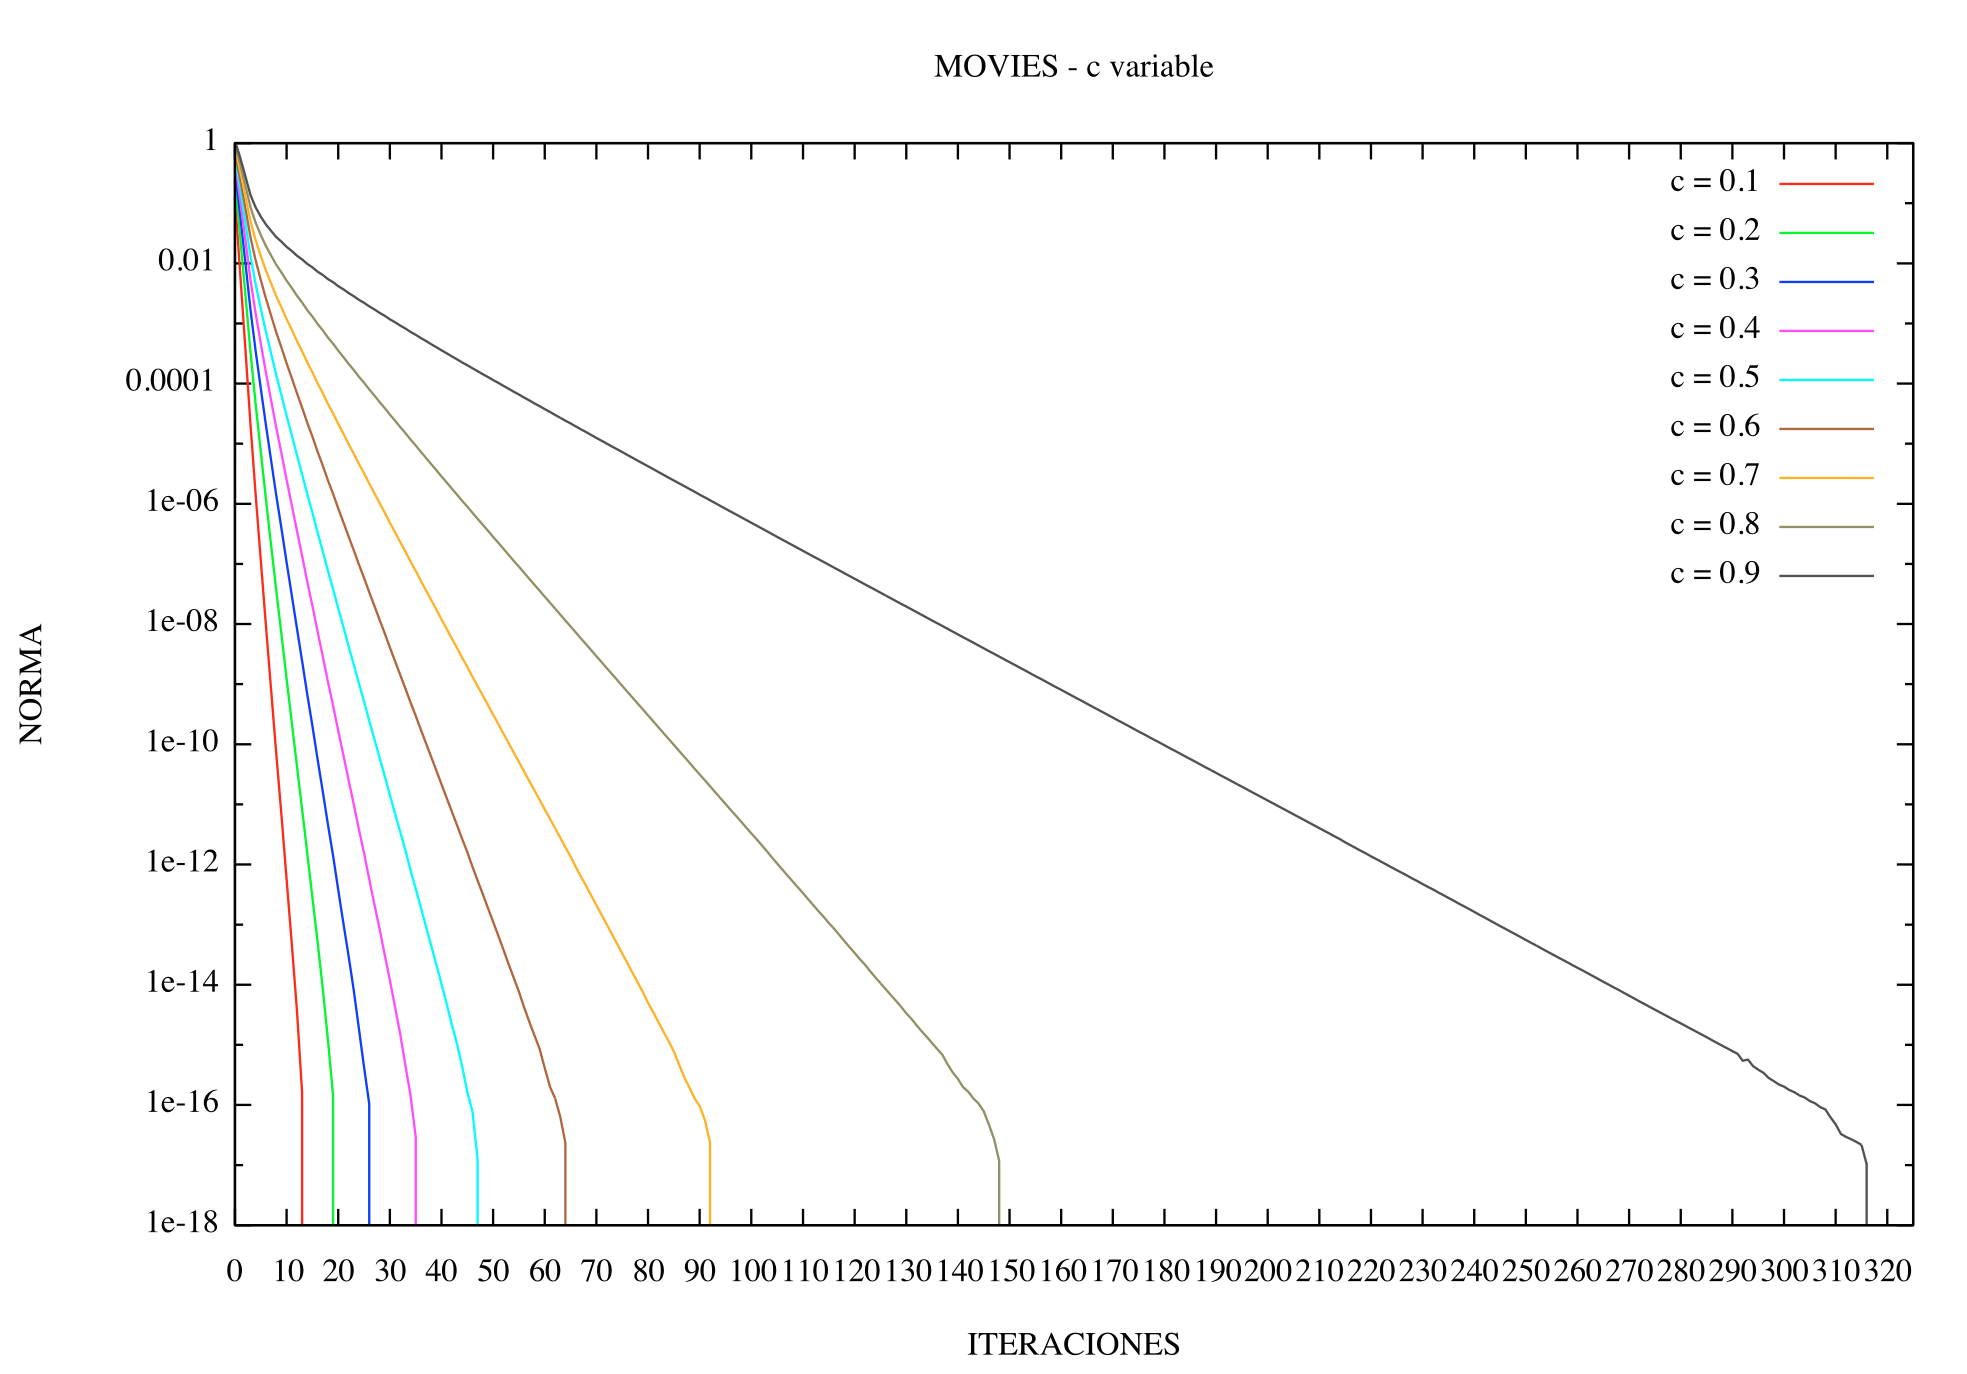
\includegraphics[scale=0.5]{imagenes/pagerank_movies_norma.png}
        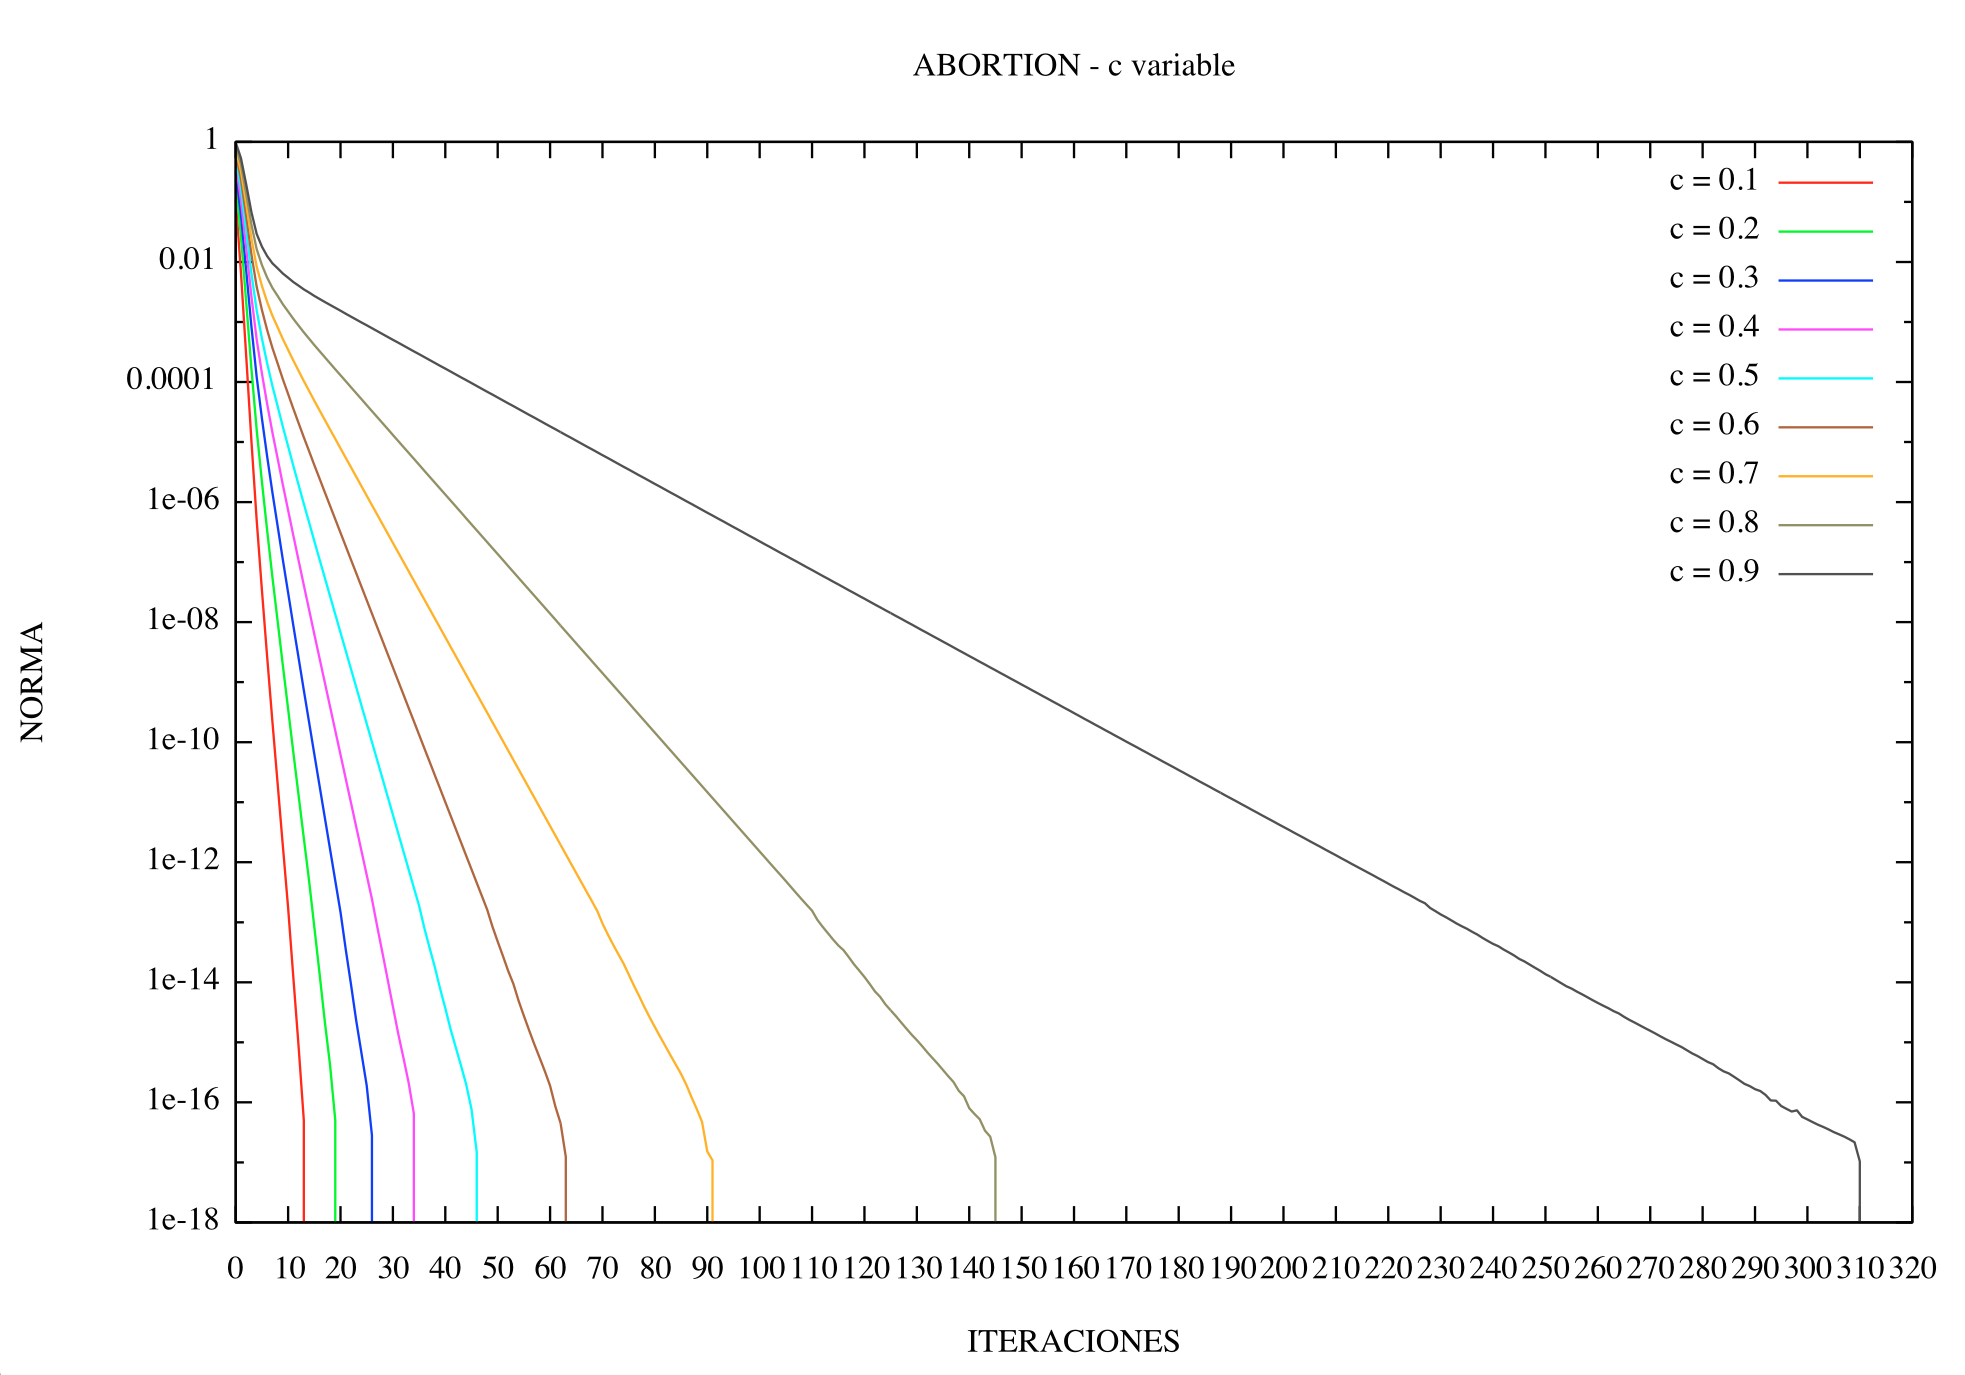
\includegraphics[scale=0.5]{imagenes/pagerank_abortion_norma.png}
       \end{center}
\end{figure}

\begin{figure}
\begin{center}
    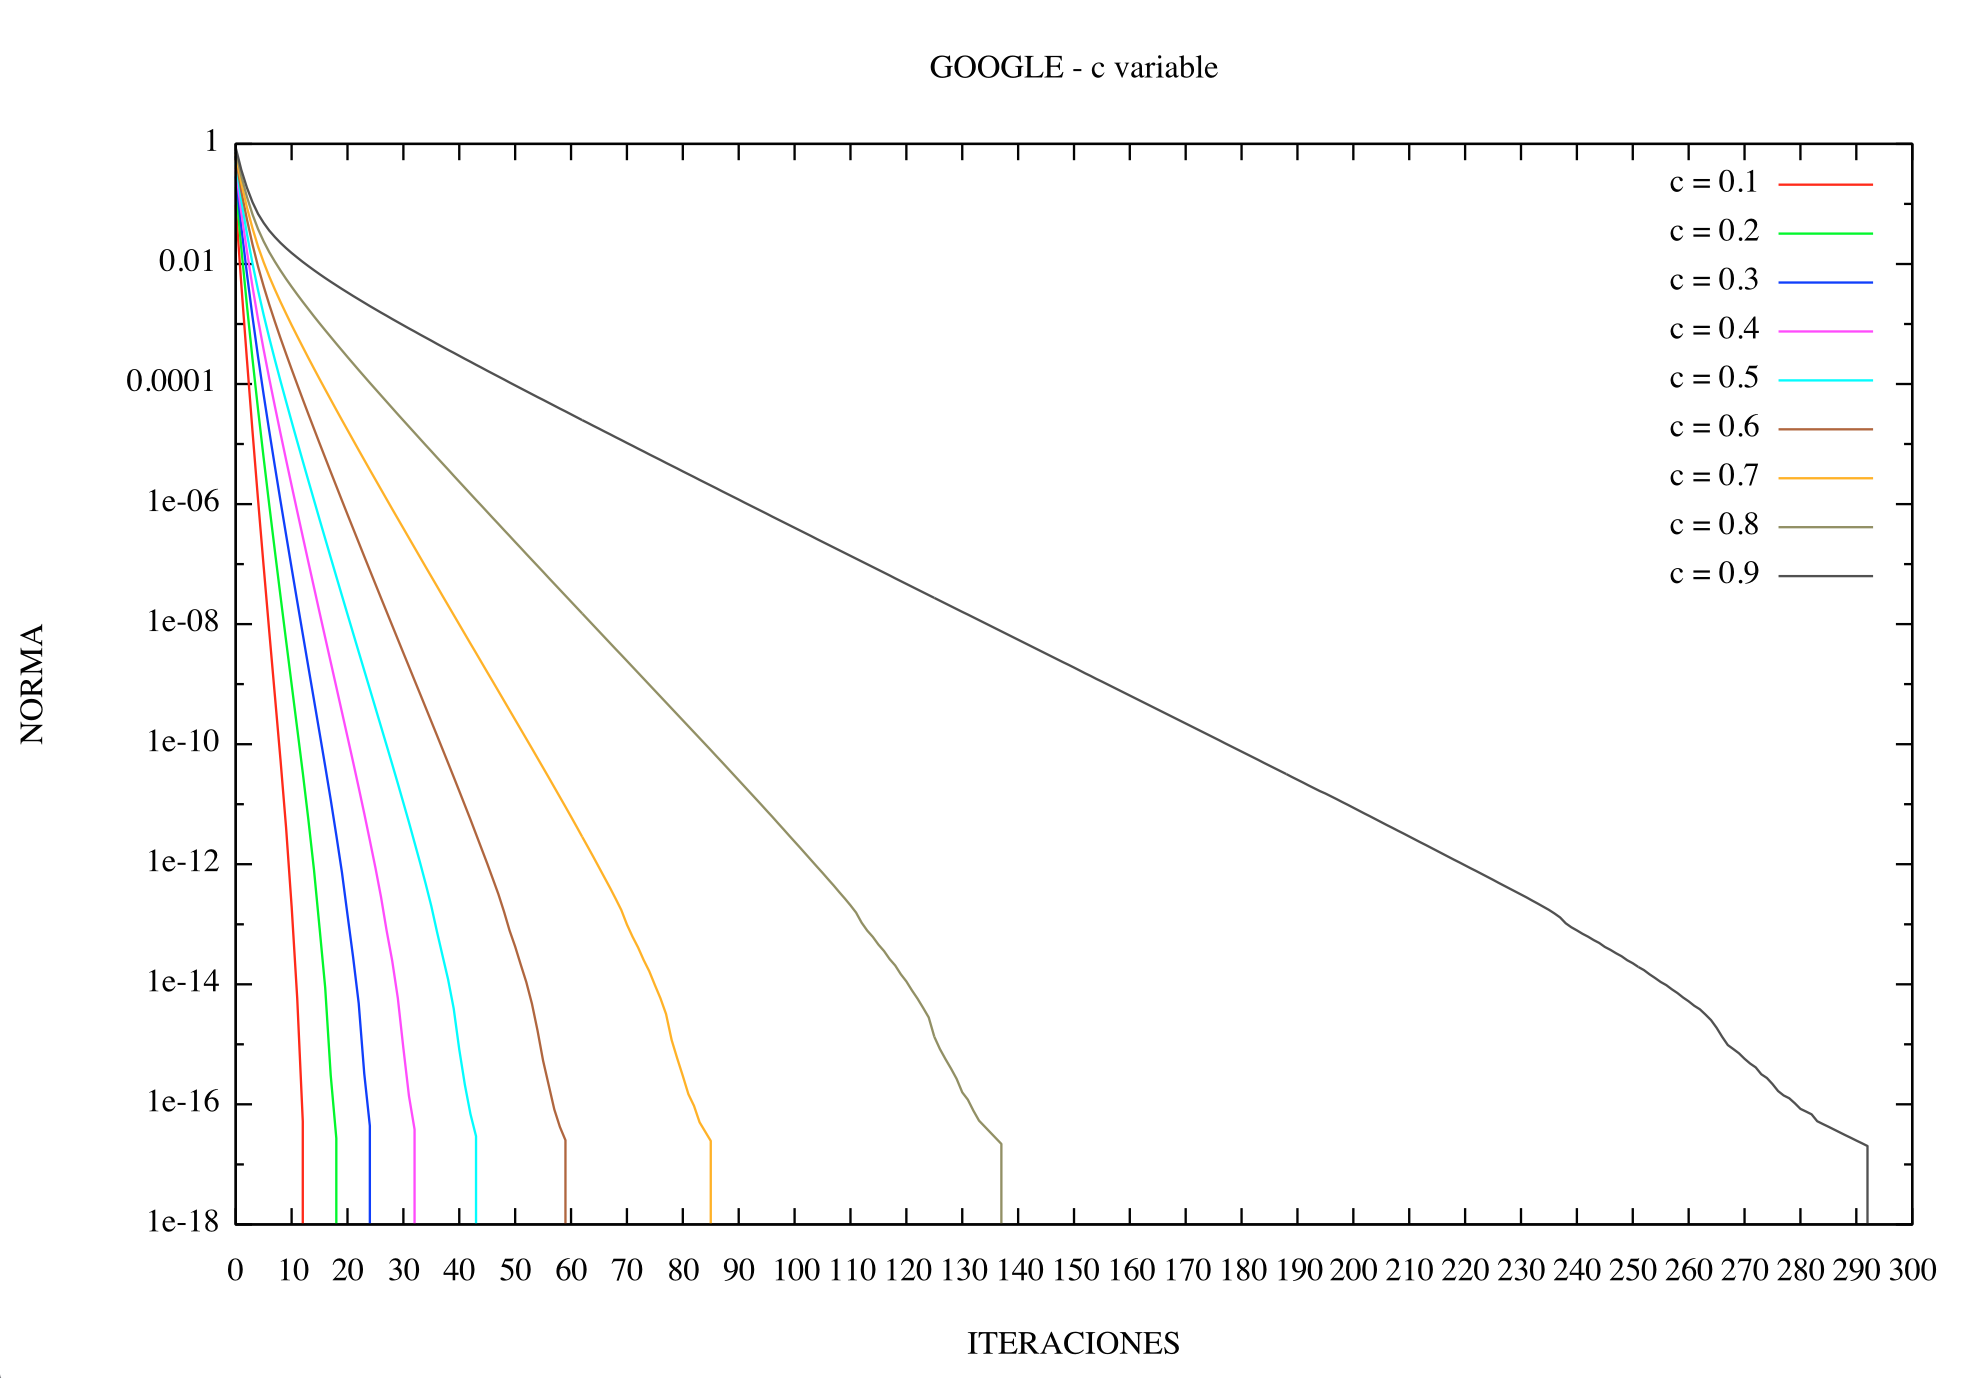
\includegraphics[scale=0.5]{imagenes/pagerank_google_norma.png}
  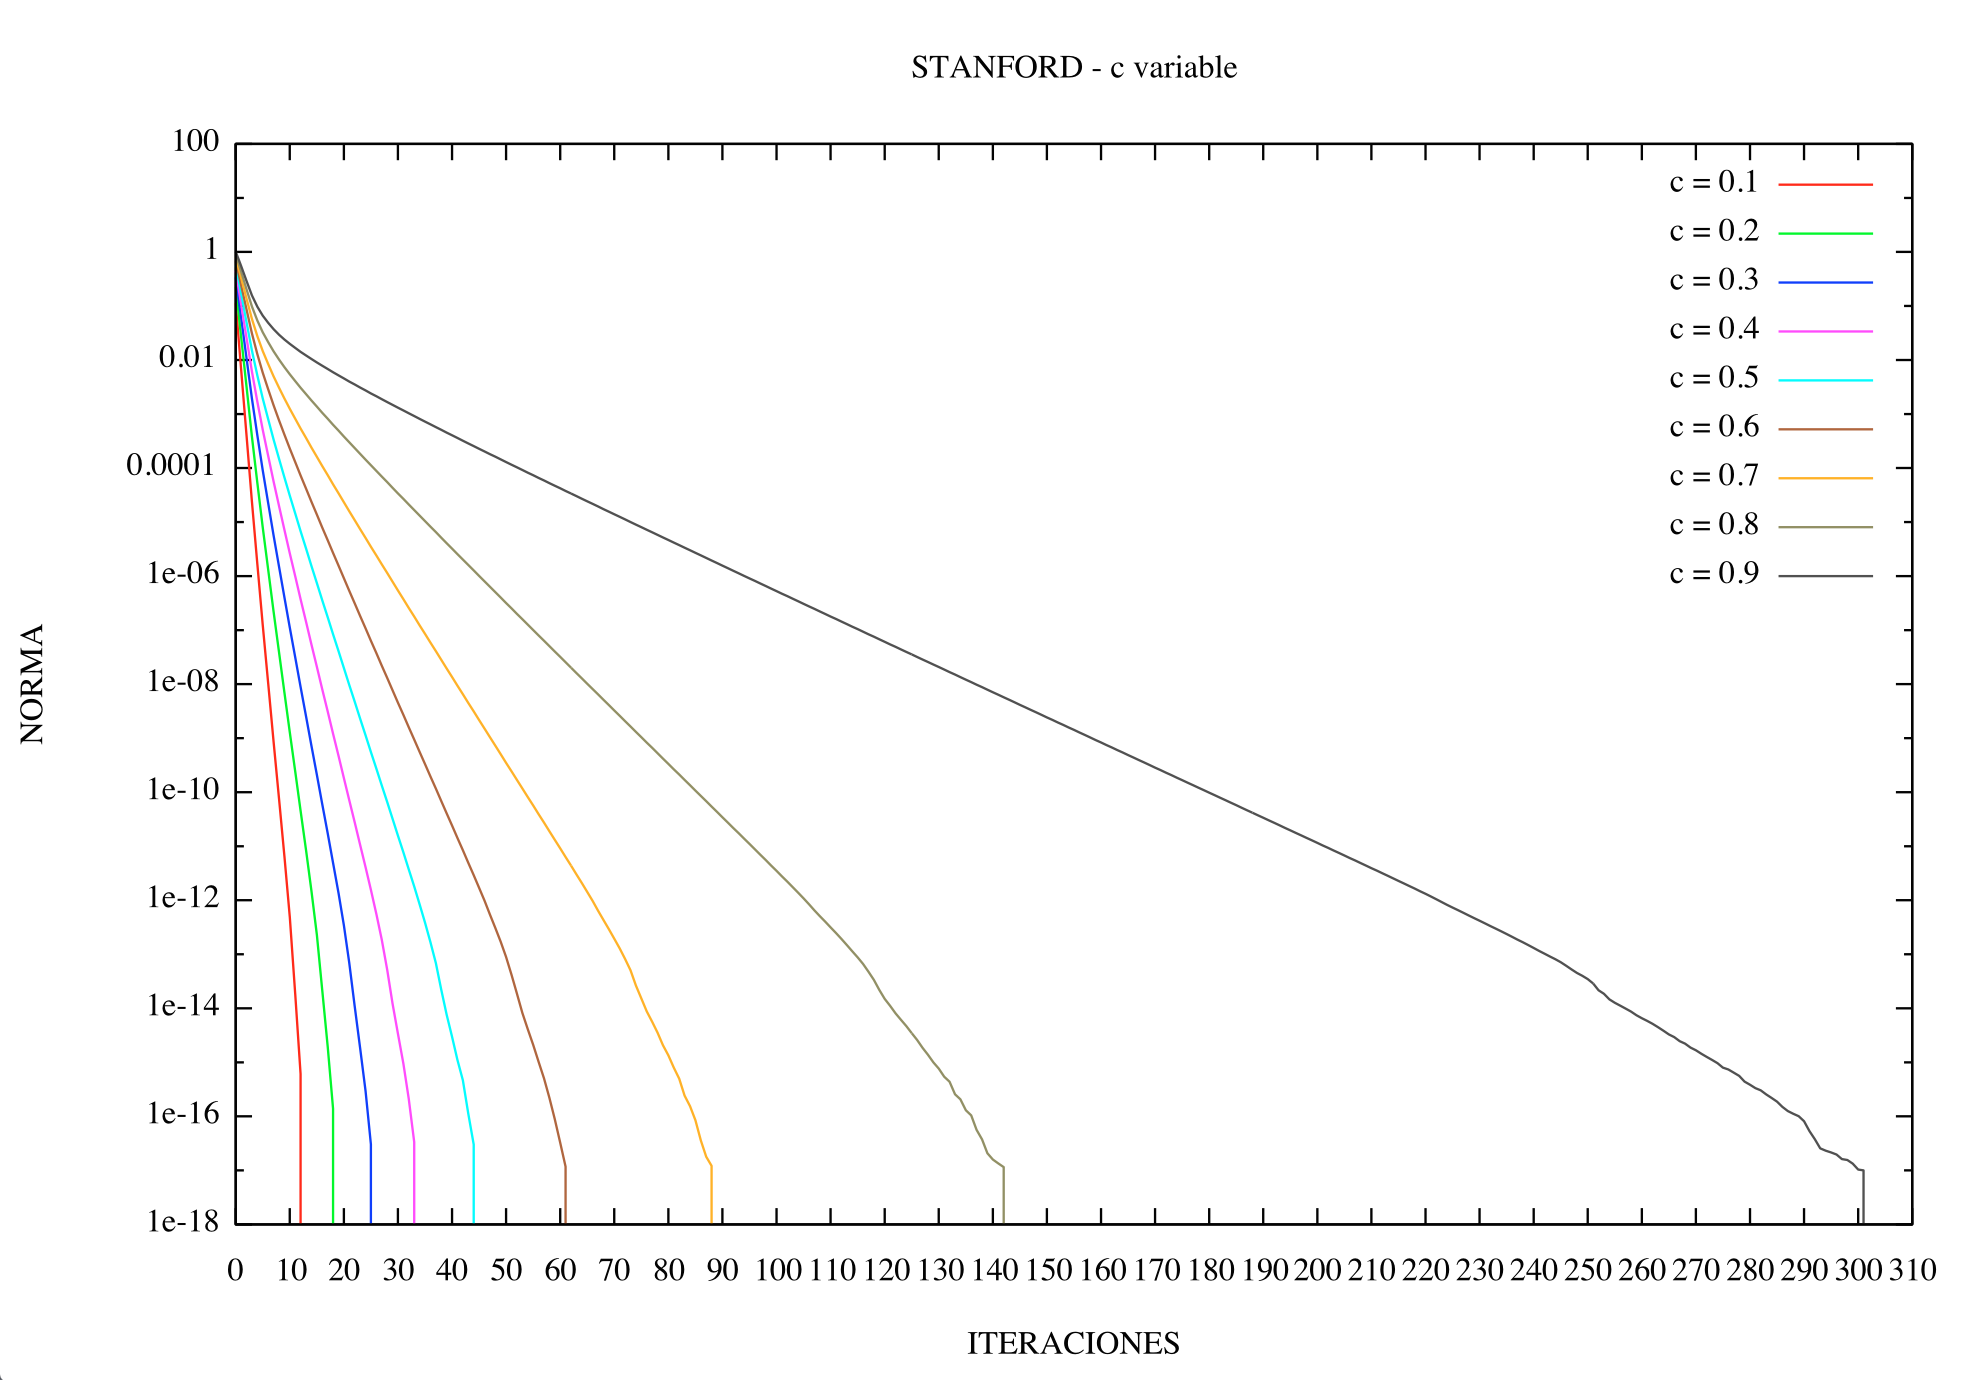
\includegraphics[scale=0.5]{imagenes/pagerank_stanford_norma.png}
    \end{center}
\end{figure}

\FloatBarrier




\subsubsection {HITS}


Estas corridas se hicieron para k= 100 ya que con esto alcanzaba para analizar los compartamientos deseados. La tolerancia en todos los casos fue de 0 ya que nos pareció mas interesante ver que tanto converge mas allá de que para nosotros una divergencia de 0.00001 ya es despreciable.

A continuación se muestran los resultados para cuatro instancias distintas, 3 medianas y una grande, de como evoluciona la norma a lo largo de las iteraciones en ambos vectores :
\begin{figure}[!htb]
\begin{center}
       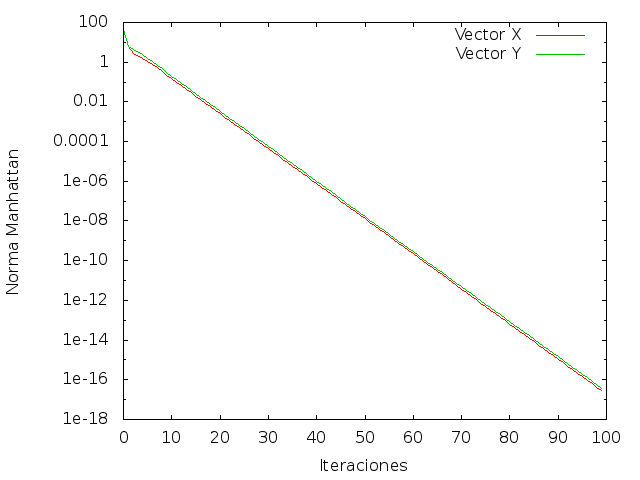
\includegraphics[scale=0.5]{imagenes/hits-abortion-expanded.png}
       \caption{Abortion expanded }
  \end{center}
\end{figure}
\begin{figure}[!htb]
\begin{center}
        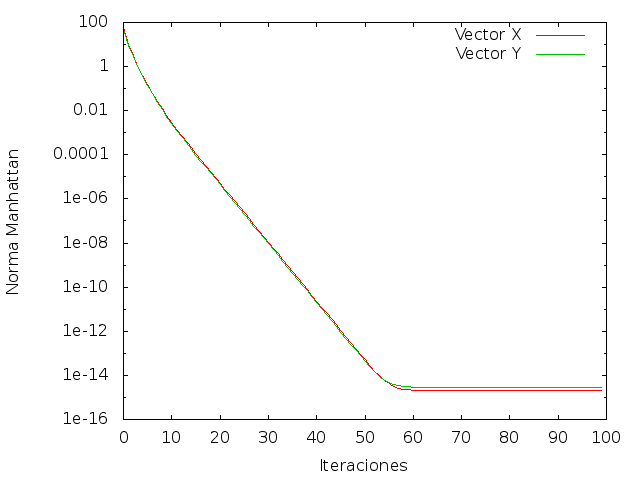
\includegraphics[scale=0.5]{imagenes/hits-genetic-expanded.png}
       \caption{Genetic expanded }
       \end{center}
\end{figure}

\begin{figure}[!htb]
\begin{center}
    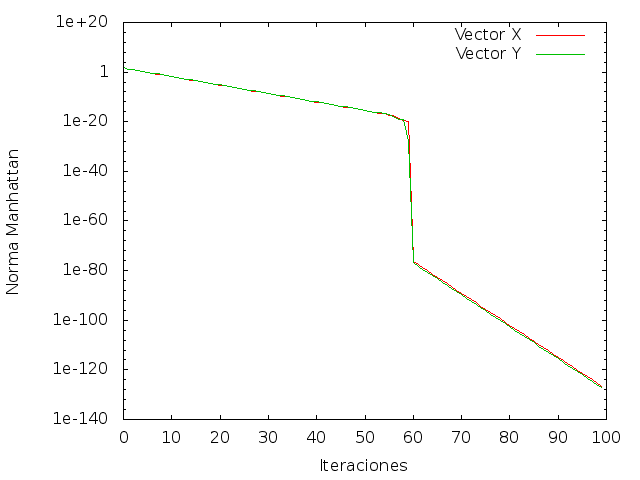
\includegraphics[scale=0.5]{imagenes/hits-movie.png}
    \caption{Movies expanded }
  \end{center}
\end{figure}
\begin{figure}[!htb]
\begin{center}
    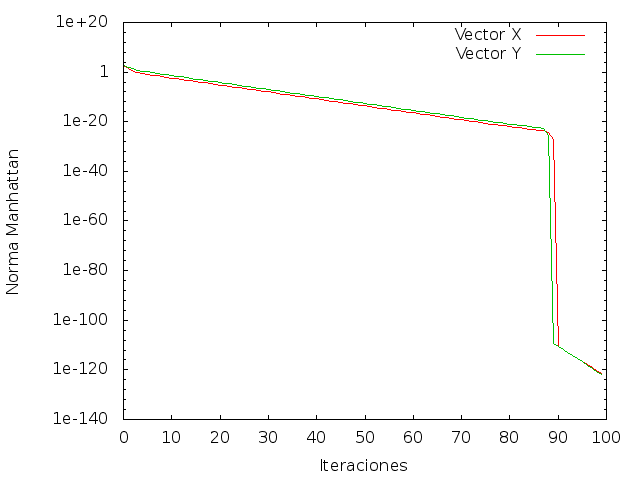
\includegraphics[scale=0.5]{imagenes/hits-stadfor.png}
    \caption{Standford}
    \end{center}
\end{figure}

\subsection{Comparación de Tiempos}

El siguiente gráfico muestra la evolución del tiempo de computo en función del tamaño de la red para cada algoritmo. La red utilizada en todos los casos es una red estrella en la que todos los nodos (o sitios) apuntan al primero de ellos. Utilizamos este tipo de grafo ya que en c++ es el más rápido y simple de crear teniendo en cuenta además que la forma del grafo no tiene un impacto de eficiencia en los algoritmos sino su tamaño en nodos y aristas es el que cambia el tiempo de ejecución. Por esto no nos pareció pertinente probar distintos tipos de grafos (arboles, completos, bipartito, etc) sin más bien el tamaño de los mismos.

 \begin{figure}[!htb]
\begin{center}
    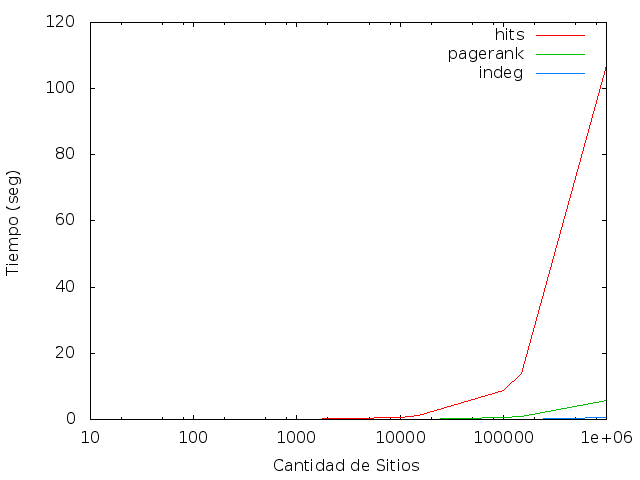
\includegraphics[scale=0.5]{imagenes/Tiempos.png}
    \caption{Tiempo de ejecución en función del tamaño de la red}
    \end{center}
\end{figure}




\newpage
\section{Discusi\'on}

\subsection{Convergencia de PageRank}
Es importante notar que para distintos tamaños de redes las iteraciones que toma para converger son muy parecidas para el mismo c. Acá solo mostramos dos ejemplos (uno grande y uno chico) pero probamos otros casos y nos dió lo mismo. \\
Así como es lo mismo para distintas redes (fijando el c), es notable como para C chicos las iteraciones son pocas, sin embargo, el crecimiento es exponencial (o más a veces) en relación al crecimiento del c. Aquí nos referimos a la cantidad de veces que realizamos el método de la potencia.

\subsection{Convergencia de HITS}
En todos los casos podemos observar que tanto el vector de hubs como el de autoridades convergen de forma muy similar, sólo en la instancia grande hay una pequeña diferencia pero es bastante despreciable. 
Por otro lado podemos ver que los casos en los que mas drásitca es la convergencia (abortion y genetic) los valores inciales de la norma manhattan son muy altos (alrrededor de 100), provocando asi que se equiparen con las que comienzan en valores mas bajos pero convergen mas lentamente (movies y standford).
En estos dos últimos casos además podemos notar grandes saltos de convergencia pasando en pocas iteracion de 1$e^{20}$ a menos de 1$e^{80}$, entiendiendo, aca sí, que la diferencia es totalmente despreciable y el valor obtenido ya ha convergido. De todas formas consideramos que puede ser un punto de interés para analizar mas en profundidad ya que más allá de decir que entendemos de eso, no sabríamos explicar porque se produce ese salto. 

\subsection{Comparación de Tiempos}

En todos los resultados el tiempo de PageRank fué menor o igual al de HITS. En los primeros dos casos (el de la cátedra y el grafo estrella) fué significativamente menor. En cambio con los grafos random se mantuvieron más cerca aunque también en muchos casos pagerank estuvo por debajo y en ninguno por arriba.\\
En el caso random podemos ver que el tiempo fluctúa, es decir, no se mantiene en crecimiento constante como el anterior. Esto es porque si bien la cantidad de nodos va creciendo puede no suceder lo mismo con la cantidad de aristas. Además, como dijimos antes, la complejidad algórtimica reside en variables desconocidas por nosotros, por lo que una instancia podría estar resultando muy compleja mientras que una mas grande mucho más simple debido a esto. De todas formas la idea de esta prueba era simplemente poder corrobar de forma mas genérica que el tiempo de cómputo de pageRank es menor al de HITS. Cosa que efectivamente podemos terminar concluyendo.\\
Finalmente cabe destacar que, como era de esperar, INDEG es la que posee menor tiempo de cómputo de forma significativa en todas las pruebas. Hasta en el caso random las distintas instancias aleatorias lo van haciendo fluctuar muy poco. Como explicamos antes esto se debe a la simplicidad algorítimca que posee.

\subsection{Comportamiento Esperado}

A continuación veremos en redes pequeñas como se comporta cada algoritmo para ver si su comportamiento es el esperado.

\subsubsection{PageRank}
Para mostrar un ejemplo del comportamiento del PageRank generamos una red de 11 nodos y lo corrimos con un $c$ = 0.85.

 \begin{figure}[!htb]
\begin{center}
    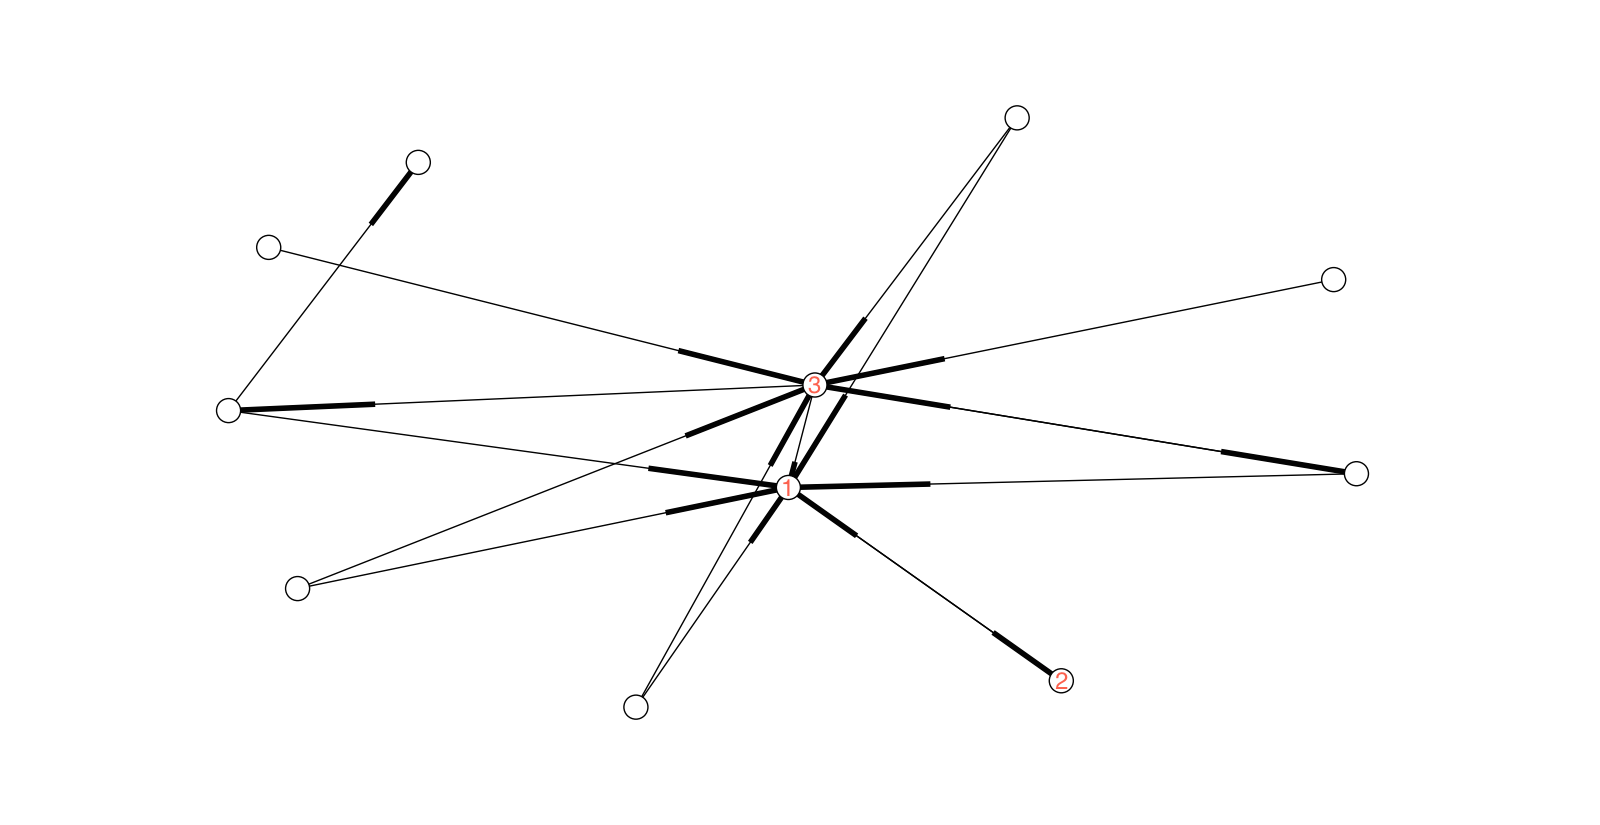
\includegraphics[scale=0.5]{imagenes/test5.png}
    \caption{Red de 11 nodos, c=0.85}
    \end{center}
\end{figure}

Lo particular de esta red es que uno $ingenuamente$ podría pensar que los dos sitios centrales 1 y 3 van a ser los que mas PageRank obtengan, pero esa suposición se basaría en que el algoritmo solo tiene en cuenta los grados de entrada de cada nodo. 
El resultado real que se obtiene de esta red es que el orden de PageRank se da por el 1, 2 y 3 (los demás nodos no son importantes para ilustrar el comportamiento). El nodo 2 le gana al 3 ya que la diferencia sustancial es que el 1 que tiene un alto valor lo apunta únicamente al 2, es decir, le da todo el peso que él tiene, mientras que el nodo 3 a pesar de tener muchos sitios que lo apuntan estos son sitios de muy bajo valor de los cuales solo tiene nodos de salida.

\subsubsection{HITS}

Dada la siguiente red, veamos que nos devuelve HITS:

 \begin{figure}[!htb]
\begin{center}
    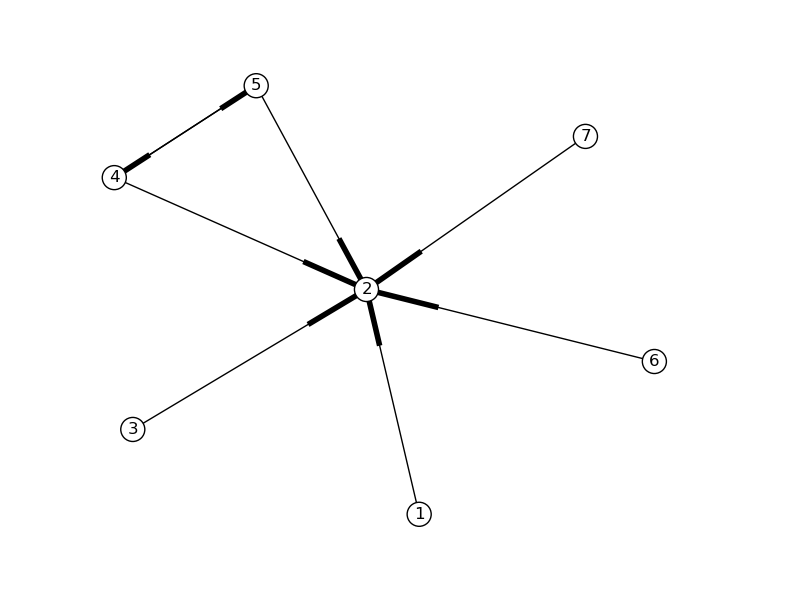
\includegraphics[scale=0.5]{imagenes/test4.png}
    \caption{Red de 7 nodos}
    \end{center}
\end{figure}

Resultado obtenido:
   $$ 
\begin{bmatrix}
              &    Autoridad  &  Hub \\
 Nodo 1 &   0.000000    &      0.383092       \\
 Nodo 2   &  0.967054    &  0.000000     \\
 Nodo 3   &  0.000000   &     0.383092  \\
 Nodo 4   &  0.180008    &     0.454401       \\
 Nodo 5   &  0.180008    &     0.454401        \\
 Nodo 6   &  0.000000    &      0.383092     \\
 Nodo 7   &  0.000000   &     0.383092 \\
\end{bmatrix} 
$$

Efectivamente podemos observar que en la columna de autoridades el nodo 2 es el mayor ya que es el que mas apuntado esta y todos aquellos que tienen 0 es porque no son apuntados por ninguno. Por otro lado en la columna de hubs podemos ver que los nodos 4 y 5 son los que mayor valor tienen ya que son los que mas apuntan a otros nodos con 2 salidas.

\subsection{Comparación de calidad}

En esta sección procederemos a discutir sobre la calidad de resultados que obtenemos de cada algoritmo y luego los compararemos entre si.\\
Como el objetivo de este trabajo práctico esta enfocado al ranking web que se le asigna a los distintos sitios de internet, consideramos como buenos resultados aquellos que aparecerían en la primer página de los buscadores, es decir, los primero 10 resultados serán los que consideraremos para el análisis.

\subsubsection{PageRank}
Según el paper de Bryan y Leise, quienes proponen el algoritmo, lo más común es que el valor del navegante aleatorio sea de 0.15. Por lo tanto creemos que con este valor es donde aparecerán los mejores resultados, pero también veremos que sucede con valores de 0.5 y 0.85, ya que estos valores indican por un lado que la probabilidad del navegante entre quedarse e irse es equiprobable y por otro lado es el inverso de lo que ellos consideran como el valor más común. En valores de 0 y 1 no tendrían sentido el análisis ya que por un lado daría la matriz original y por el otro una matriz equiprobable.\\
El caso de prueba que utilizaremos es el dado por la cátedra, \textbf{Death Penalty}, y lo elegimos ya que es un tema bastante discutido donde se pueden encontrar resultados interesantes.


\paragraph{Resultados con un c=0.15}
\begin{enumerate}
\item
http://www.amnesty.org\\
Amnesty International On-line: human rights website\\
\item
http://www.quaker.org/fcadp\\
Friends Committee to Abolish the Death Penalty\\
\item
\textbf{No relacionado con el tema}\\
http://www.santegidio.org/solid/pdm/pdm.htm\\
Sito spostato\\
\item
http://www.aclu.org/issues/death/hmdp.html\\
Death Penalty and the ACLU\\
\item
http://sun.soci.niu.edu/~critcrim/dp/dp.html\\
Death Penalty Information (from: http://www.soci.niu.edu/~critcrim)\\
\item
http://www.ncadp.org
National Coalition To Abolish the Death Penalty
\item
http://www.ccadp.org
Canadian Coalition Against the Death Penalty
\item
http://www.deathpenalty.org
Death Penalty Focus
\item
http://www.smu.edu/~deathpen
Death Penalty News \& Updates
\item
http://www.derechos.org/dp
Death Penalty Links
% \item
 % \textbf{No relacionado con el tema}\\
% http://www.allexperts.com/about.asp\\
% AllExperts.com
% \item
% http://www.nrlc.org\\
% National Right to Life Organization
% \item
% \textbf{No relacionado con el tema}\\
% http://www.phone-soft.com/at/cyber-world/international/o1480i.htm\\
% PHONE-SOFT INTERNET DIRECTORY INTERNATIONAL:HERB THERAPY LINKS
% \item
% http://www.lm.com/~jdehullu\\
% Ariadne's Thread: On abortion, affirmative action, hate speech
% \item
% http://www.plannedparenthood.org\\
% Planned Parenthood Federation of America
% \item
% http://www.gynpages.com\\
% Abortion Clinics OnLine
% \item
% http://www.care-net.org/link.htm\\
% CareNet Links
% \item
% http://www.naral.org\\
% NARAL: Abortion and Reproductive Rights: Choice For Women
 % \item
% http://www.crosswalk.com/ftr/1,,17,00.htm \\
% Crosswalk.com Forums - Welcome
 % \item
% http://www.cais.com/agm/main\\
% The Abortion Rights Activist Home Page

\end{enumerate}

\paragraph{Resultados con un c=0.5}
 \begin{enumerate}
 \item
http://www.amnesty.org\\
Amnesty International On-line: human rights website\\
\item
http://www.quaker.org/fcadp\\
Friends Committee to Abolish the Death Penalty\\
\item
\textbf{No relacionado con el tema}\\
http://www.santegidio.org/solid/pdm/pdm.htm\\
Sito spostato\\
\item
http://www.aclu.org/issues/death/hmdp.html\\
Death Penalty and the ACLU\\
\item
\textbf{No relacionado con el tema}\\
http://www.web.amnesty.org/rmp/dplibrary.nsf/index?openview\\
Empty title field\\
\item
http://sun.soci.niu.edu/~critcrim/dp/dp.html\\
Death Penalty Information (from: http://www.soci.niu.edu/~critcrim)\\
\item
http://www.ccadp.org\\
Canadian Coalition Against the Death Penalty\\
\item
http://www.ncadp.org\\
National Coalition To Abolish the Death Penalty\\
\item
http://www.smu.edu/~deathpen\\
Death Penalty News \& Updates\\
\item
http://www.derechos.org/dp\\
Death Penalty Links\\


 % \item http://www.allexperts.com/about.asp\\
% AllExperts.com
 % \item http://www.nrlc.org\\
% National Right to Life Organization
 % \item \textbf{No relacionado con el tema}\\
 % http://home.about.com\\
% About - The Human Internet
 % \item \textbf{No relacionado con el tema}\\
% http://www.phone-soft.com/at/cyber-world/international/o1480i.htm\\
% PHONE-SOFT INTERNET DIRECTORY INTERNATIONAL:HERB THERAPY LINKS
 % \item http://www.lm.com/~jdehullu\\
% Ariadne's Thread: On abortion, affirmative action, hate speech
 % \item http://www.plannedparenthood.org\\
% Planned Parenthood Federation of America
 % \item http://www.care-net.org/link.htm\\
% CareNet Links
 % \item http://www.gynpages.com\\
% Abortion Clinics OnLine
 % \item http://www.marchforlife.org\\
% The March For Life Fund Home Page
 % \item \textbf{No relacionado con el tema}\\
% http://www.jbs.org\\
% The John Birch Society
 \end{enumerate}
 
\paragraph{Resultados con un c=0.85}
 \begin{enumerate}

\item
http://www.amnesty.org\\
Amnesty International On-line: human rights website\\
\item
\textbf{No relacionado con el tema}\\
http://www.web.amnesty.org/rmp/dplibrary.nsf/index?openview\\
Empty title field\\
\item
http://www.quaker.org/fcadp\\
Friends Committee to Abolish the Death Penalty\\
\item
\textbf{No relacionado con el tema}\\
http://notes.nacdl.org\\
Access to Members Only Areas\\
\item
http://www.criminaljustice.org\\
National Association of Criminal Defense Lawyers On-line\\
\item
\textbf{No relacionado con el tema}\\
http://www.ewg.org\\
Environmental Working Group\\
\item
\textbf{No relacionado con el tema}\\
http://www.santegidio.org/solid/pdm/pdm.htm\\
Sito spostato\\
\item
http://www.aclu.org/issues/death/hmdp.html\\
Death Penalty and the ACLU\\
\item
http://sun.soci.niu.edu/~critcrim/dp/dp.html\\
Death Penalty Information (from: http://www.soci.niu.edu/~critcrim)\\
\item
\textbf{No relacionado con el tema}\\
http://www.ablexbooks.com\\
Ablex Publishing Welcome Page\\

 % \item 
 % \textbf{No relacionado con el tema}\\
 % http://www.jbs.org\\
% The John Birch Society
 % \item 
 % \textbf{No relacionado con el tema}\\
% http://home.about.com\\
% About - The Human Internet
 % \item 
 % \textbf{No relacionado con el tema}\\
% http://www.allexperts.com/about.asp\\
% AllExperts.com
 % \item
  % \textbf{No relacionado con el tema}\\
% http://www.aobs-store.com\\
% American Opinion Book Services Online Store
 % \item
% http://www.nrlc.org\\
% National Right to Life Organization
 % \item 
 % \textbf{No relacionado con el tema}\\
% http://www.trimonline.org\\
% TRIMonline - Lower Taxes Through Less Government
 % \item
% http://www.marchforlife.org\\
% The March For Life Fund Home Page
 % \item 
 % \textbf{No relacionado con el tema}\\
% http://www.phone-soft.com/at/cyber-world/international/o1480i.htm\\
% PHONE-SOFT INTERNET DIRECTORY INTERNATIONAL:HERB THERAPY LINKS
 % \item 
% \textbf{No relacionado con el tema}\\
% http://www.reagan.com\\
% The Reagan Information Interchange
 % \item 
 % \textbf{No relacionado con el tema}\\
% http://www.pregnancycenters.org\\
% Pregnancy Centers Online
 \end{enumerate}

En base a los resultados se puede ver como a medida que aumenta el $c$ empiezan a aparecer resultados que poco tienen que ver con el tema directamente, ya que puede estar relacionado de alguna forma o no diferenciarse tanto del eje temático.\\
Nos pareció extraño que aparece siempre muy bien posicionado el sitio web Sito spostato, que nada tiene que ver con el tema de la pena de muerte, por lo tanto decidimos hacer un foco especial en este para ver porque sucedía esto y llegamos a la conclusión que es debido a que el factor mas determinante es que gran cantidad de sitios referidos al tema y a su vez bien posicionados (aunque fuera del top 10) apuntaban al mismo, y por lo tanto le daban bastante peso a Sito spostato.\\
Aunque se pueda ver que con un $c$ menor los resultados tienen relación con el tema, deja claro que sitios como Google o todos aquellos que utilicen este tipo de algoritmos, trabajan bastante sobre el resultado del algoritmo para eliminar sitios de SPAM o mejorar la calidad todavía más.

\subsubsection{HITS}
Este analásis de calidad lo haremos sobre el tema death penalty. Veremos cuales son los primeros 5 resultados que devuelve HITS en cuanto a autoridades y hubs.

% \paragraph{Resultados Autoridades}
% \begin{enumerate}
% \item
% 0.33395\\
% 957 (1184) [O]\\
% http://www.amazon.com/exec/obidos/redirect-home/youdebatecom\\
% Amazon.com--Earth's Biggest Selection\\

% \item
% 0.33395\\
% 938 (1165) [O]\\
% http://www5.dimeclicks.com\\
% DimeClicks.com - Complete Web and Marketing Solutions\\

% \item
% 0.33395\\
% 966 (1193) [O]\\
% http://rd1.hitbox.com/rd?acct=WQ590703J6FB45EN5\\
% HitBox.com - hitbox web site traffic counter - internet statistics and site promotion tools - WebSideStory\\

% \item
% 0.33296\\
% 960 (1187) [O]\\
% http://www.amazon.com/exec/obidos/redirect?tag=youdebatecom\&amp;path=subst/electronics/misc/top-sellers.html\\
% Amazon.com--Earth's Biggest Selection\\

% \item
% 0.33296\\
% 961 (1188) [O]\\
% http://www.amazon.com/exec/obidos/redirect?tag=youdebatecom\&path=subst/electronics/software/home.html\\
% Amazon.com Software\\

% \end{enumerate}


% \paragraph{Resultados Hubs}
% \begin{enumerate}
% \item
% 0.09569\\
% 47 (48) [R]\\
% http://www.4greatbooks.com/abortion-books.htm\\
% Abortion Books Pro and Con\\
% 
% \item
% 0.09428\\
% 1005 (1232) [O]\\
% http://www.youdebate.com/government.htm\\
% Government Debates and Polls\\
% 
% \item
% 0.09428\\
% 1006 (1233) [O]\\
% http://www.youdebate.com/POLITICS.htm\\
% Political Debates and Polls\\

% \item
% 0.09428\\
% 1020 (1247) [O]\\
% http://www.youdebate.com/UNITEDSTATES.htm\\
% United States debates\\

% \item
% 0.09410\\
% 1019 (1246) [O]\\
% http://www.youdebate.com/Presidentialcontenders.htm\\
% Presidential Contenders Debates and Polls\\

% \end{enumerate}


\paragraph{Resultados Hubs}
\begin{enumerate}
\item
http://www.clarkprosecutor.org/html/links/dplinks.htm\\
Death Penalty Links
\item
http://faculty.etsu.edu/blankenm/deathlinks.htm\\
Death Penalty Links
\item
http://coramnobis.com/portal/deathpen.html\\
A Capital Defender's Toolbox: criminal defense  death penalty litigation online resource center
\item
http://info-s.com/deathpenalty.html\\
The Info Service
\item
http://members.xoom.com/ccadp/links.htm\\
Canadian Coalition Against the Death Penalty - Collection of Links
\end{enumerate}

\paragraph{Resultados Autoridades}
\begin{enumerate}
\item
http://sun.soci.niu.edu/~critcrim/dp/dp.html\\
Death Penalty Information
\item
http://www.aclu.org/issues/death/hmdp.html\\
Death Penalty and the ACLU
\item
http://www.ncadp.org\\
National Coalition To Abolish the Death Penalty
\item
http://www.smu.edu/~deathpen\\
Death Penalty News and Updates
\item
http://www.deathpenalty.org\\
Death Penalty Focus
\end{enumerate}

Aquí podemos observar claramente que la calidad además de ser, a priori, buena y correcta, tiene coherencia. La mayoría de los hubs sobre el tema son conjunto de links sobre pena de muerte, servicios de información o 
central de recursos sobre litigios en penas de muerte. Por otro lado, las autoridades son diarios con noticias y novedades, organizaciones enfocadas a eso o páginas institucionales (.edu). Ambos tienen sentido en sus 
categorías ya que es totalmente lógico que páginas institucionales sean fuentes propias de información que son citadas por otras (osea autoridades) o que una central de recursos linkee a muchos otros citios (osea un hub).\\
También es de destacar que ningún link pareciera ser spam, o sobre algo no relacionado.

\subsubsection{Comparación de calidad}

Si comparamos los resultados del PageRank con un $C$ alto claramente da mejores respuestas el HITS. Sin embargo en el paper de Bryan y Leise$[3]$ se recomienda un $C$ de 0.15, con este valor los resultados mejoran notoriamente aunque sigue habiendo algunos que no corresponden o son SPAM. 
Bajo este ejemplo podemos notar que tienen resultadoes muy similares, aunque Page Rank tiene SPAM en su resultado y HITS no. Esto tiene sentido en la medida que el mismo paper de HITS recomienda el uso de su algoritmo en sets chicos y a priori parece tener mejor resultado HITS. Esto a su vez es subjetivo pero nos parece interesante que sitios que parecen representar bien el tema como http://www.deathpenalty.org y http://www.ncadp.org aparecen en ambos resultados.


\newpage

\section{Conclusiones}

\subsection{PageRank}
Este algoritmo resultó bastante sencillo de implementar, una gran parte del mismo fue la implementación de la matriz esparsa para mejorar tanto la performance espacial como la temporal en el cálculo del método de la potencia. \\
En cuanto a tiempos es bastante estable y podemos deducir bajo las pruebas realizadas que debería seguir siendo así para grafos aún más grandes. A contrapartida, la calidad si bien es muy buena para c$=$0.15, lo que confirma el comentario en el paper original, notamos que hay un trabajo grande por encima en los buscadores reales pero es un muy buen punto de partida. Nos referimos a posicionamiento por publicidad, eliminación de SPAM, etc.

\subsection{HITS}

Una parte importante sobre este algoritmo es que tarda mucho para nodos grandes, sin embargo no debemos olvidar que en su paper$[2]$ Kleinberg habla de que este algoritmo debe ser aplicado no sobre toda la red sin sobre un subconjunto de la misma ($\textit{root set}$) obtenido de una busqueda incial. Por lo tanto si acotamos el análisis a los grafos mas acotados podemos ver que el tiempo de computo es aceptable y hasta muy parecido al de page rank. 

\subsection{INDEG}

Este algoritmo es bastante simple y en una red chica y confiable puede llegar a valer. Es muy rápido y en caso de necesitar algún dato rápido, es muy fácil de implementar. Igualmente tiene mucho peso la confiabilidad, ya que es muy simple de crecer tu puntaje, simplemente comprando un lugar mínimo en la mayor cantidad de páginas posibles.

%  \begin{figure}[!htb]
% \begin{center}
%     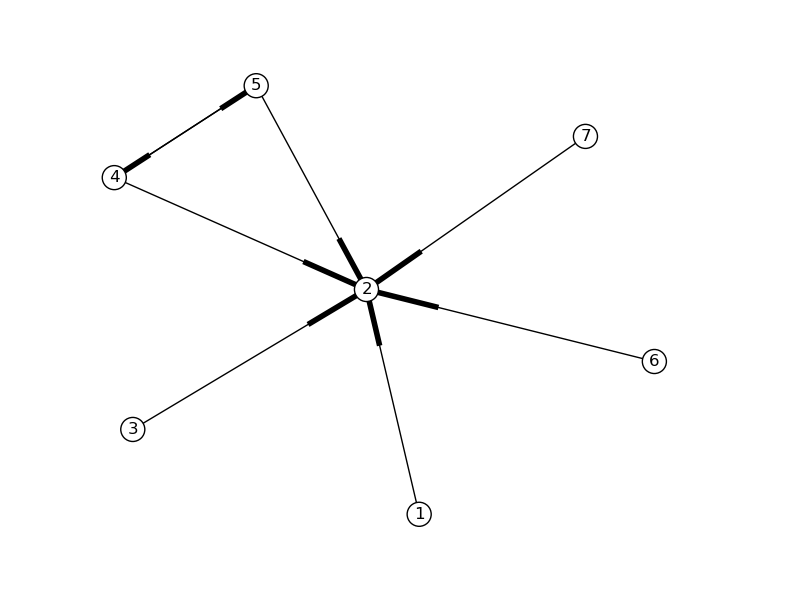
\includegraphics[scale=0.5]{imagenes/test4.png}
%     \caption{Red de 7 nodos}
%     \end{center}
% \end{figure}

% \subsection{Mejor estrategia para comprar links}
% \subsubsection{PageRank}

% Como explicamos anteriormente, el algoritmo de PageRank prioriza la calidad del sitio de entrada antes que la cantidad. Por lo tanto supongamos que tenemos el siguiente escenario:


%  \begin{figure}[!htb]
% \begin{center}
%     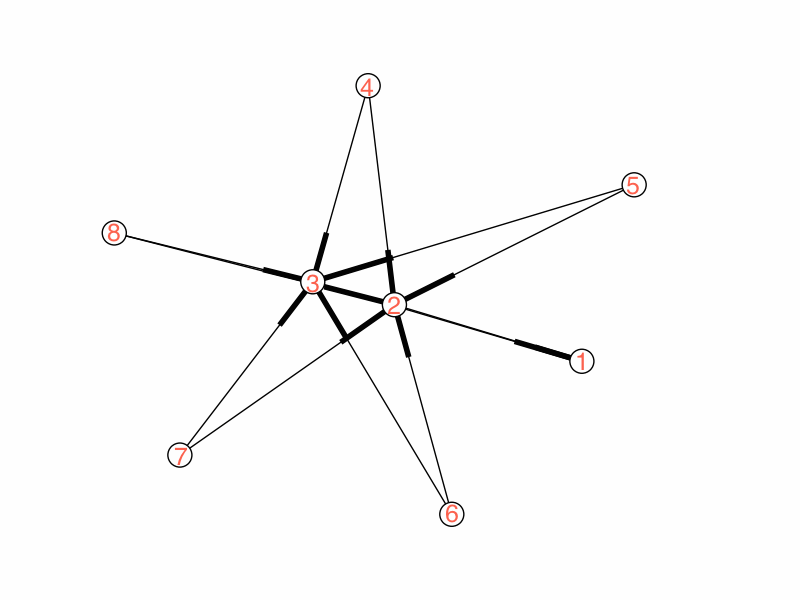
\includegraphics[scale=0.5]{imagenes/test6.png}
%     \caption{Red de 8 nodos, c=0.85}
%     \end{center}
% \end{figure}

% Cuyos pesos son:
%    $$ 
% \begin{bmatrix}
% Nodo 1 & 0.32079\\
% Nodo 2 & 0.15762\\
% Nodo 3 & 0.15762\\
% Nodo 4 & 0.05283\\
% Nodo 5 & 0.05283\\
% Nodo 6 & 0.05283\\
% Nodo 7 & 0.05283\\
% Nodo 8 & 0.05283\\
% \end{bmatrix} 
% $$

% Ahora, suponiendo que el costo de cada nodo es mas caro a medida que aumenta su peso, vamos a ver que es más conveniente, si comprar el derecho a que el nodo 1 nos apunte o en vez de eso comprar el linkeo de los nodos 2 y 3. Entonces vamos a testear como se comporta el algoritmo mediante estas dos alternativas lineando al sitio de los Wachiturros.


%    $$ 
% \begin{bmatrix}
%  & Nodo 1 & Nodo 2 y 3 \\
% Wachiturros & 0.24557  & 0.05018   \\
% Nodo 1 & 0.24201& 0.30469\\
% Nodo 2 & 0.11891& 0.14971\\
% Nodo 3 & 0.11891& 0.14971\\
% Nodo 4 & 0.03986  & 0.05018\\
% Nodo 5 & 0.03986  & 0.05018\\
% Nodo 6 & 0.03986  & 0.05018\\
% Nodo 7 & 0.03986 & 0.05018\\
% Nodo 8 & 0.03986 & 0.05018\\
% \end{bmatrix} 
% $$

% Por lo tanto se puede ver que conviene que el Nodo 1 nos apunte antes que el 2 y 3. Conviene porque nos asigna un mayor peso y porque nos deja a su vez mejor posicionado en la tabla final. Además de significar una optimización en el costo total.

\subsubsection{HITS}
Si el algoritmo aplicado en la red fuese HITS lo recomendable al cliente sería que negocie con los principales HUBS para que apunten a su sitio. Logrando así rankear mejor en la sección de Autoridades sobre el tema. 
No le recomendaríamos que negocie con las páginas autoridades ya que dificilmente estas accediesen debido a que de esta manera se estarían restando puntos en el ranking de autoridades.\\
Por ejemplo en el caso de death penalty habría que negociar con alguno de los 3 principales HUBS: clarkprosecutor.org, faculty.etsu.edu o coramnobis.com. Teniendo en cuenta el costo de cada uno, ya que si el primero costase el doble 
o mas que el segundo tal vez convendría más negociar con el segundo y tercero.

\begin{thebibliography}{9}

\bibitem{fpedrochev}
  $http://personales.upv.es/~pedroche/inv/_docs/fpedrochev4(sema).pdf$

\bibitem{Kleinberg}
$Jon M. Kleinberg. Authoritative sources in a hyperlinked environment. J. ACM,
46(5):604,632, September 1999.$

\bibitem{Bryan y Leise}
$Kurt Bryan and Tanya Leise. The linear algebra behind google. SIAM Review, 48(3):569
581, 2006.$

\bibitem{Burden y Faires}
$Burdan y Faires, Numerical Analysis, 3rd edition, 453
467, 2002.$


\end{thebibliography}

\newpage

\end{document}

